%% ============================================================
%% 分片 22：原文第 9 节「't Hooft And Hecke Operators」（原文 glshort.tex 起于第 6755 行）
%% 由 tools/harvmac2tex.py 从 arXiv 源码（hep-th/0604151v3）自动生成。
%% 只译英文散文；公式、编号、\label、\cite 一律不改。
%% ============================================================

\section{'t Hooft And Hecke Operators}
\label{sec:thooftheckeop}

 The goal of the present section is to begin the study of
the supersymmetric 't Hooft operators that appear at $\Psi=0$, a
value we reach by setting $t=1$ and $\theta=0$.  The main result
will be to show that 't Hooft operators correspond to the Hecke
operators of the geometric Langlands program.

We will mainly consider static 't Hooft operators. So our
four-manifold will be $M=\Bbb{R}\times W$, for some three-manifold
$W$, and our 't Hooft line operators will be supported on
one-manifolds of the form $\Bbb{R}\times p$, for some point $p\in
W$.  As we have discussed in section 第~\ref{sec:loopop}~节, line ``operators''
of this kind are not operators in the usual sense, acting on a
pre-existing vector space; rather, they must be incorporated in
the definition of the space of physical, supersymmetric states.

Our four-dimensional TQFT at $\Psi=0$ reduces in two dimensions to
the $A$-model with target $\MH$ in complex structure $K$.  So let
us first recall some facts about $A$-models.  In general, in a
two-dimensional $A$-model with target $X$, a supersymmetric
classical field configuration is a holomorphic map $\Phi:\Sigma\to
X$. Moreover, the first approximation to the space of
supersymmetric states is the cohomology of the space of
time-independent supersymmetric classical fields on
$\Sigma=\Bbb{R}\times I$, with $I$ being an interval.
Supersymmetric fields are holomorphic maps  $\Phi:\Sigma\to X$.
But a holomorphic map that is also time-independent is necessarily
a constant. So in the $A$-model, the classical approximation to
the space of physical states is simply the cohomology of the space
of constant maps to $X$ that obey the boundary conditions.   For
example, in Floer theory, one takes boundary conditions such that
the two boundary components of $\Bbb{R}\times I$ are mapped to two
specified Lagrangian submanifolds $N,N'\subset X$. A constant map
with these boundary conditions must map $\Sigma$ to the
intersection $N\cap N'$, so the classical approximation to the
space of supersymmetric states is simply the cohomology of $N\cap
N'$.  (One must shift the dimensions or ghost numbers of the
cohomology classes in order to account for the number of filled
fermion states in the vacuum. Mathematically, the shift involves
the Maslov index.)

In general, there are instanton corrections to this classical
intersection; their study is the main content of Floer theory. But
we will see that for the branes we consider, there are no
instanton corrections to the $A$-model at $\Psi=0$; the
supersymmetric configurations are all time-independent.

\par\medskip{\it Reduction To Two Dimensions}

Aiming to reduce to a two-dimensional model on $ \Bbb{R}\times I$,
we specialize our four-manifold, which so far has been
$M=\Bbb{R}\times W$,  by taking $W=I\times C$, where $C$ is a
Riemann surface and $I$ an interval at whose ends we take boundary
conditions defined by choices of brane.  So altogether, we work on
$M=\Bbb{R}\times I\times C$. The conditions for supersymmetry are
familiar from section 第~\ref{sec:familya}~节:
% 式 (9.1)
\setcounter{equation}{0}
\begin{equation}\label{eq:oops}
\begin{aligned}(F-\phi\wedge\phi+tD\phi)^+ & = 0 \\
                      (F-\phi\wedge\phi-t^{-1}D\phi)^-& = 0 \\
                      D^* \phi & = 0.\\\end{aligned}
\end{equation}

At $t=1$, which we generally assume in our study of 't Hooft
operators, the first two equations in \eqref{eq:oops}\ can be written
$F-\phi\wedge \phi+\star D\phi=0$.  In terms of the complex
connection $\CA=A+i\phi$ and curvature $\CF=d\CA+\CA\wedge\CA$,
this is equivalent to % 式 (9.2)
\setcounter{equation}{1}
\begin{equation}\label{eq:nops}
{\cal F}+i\star\bar\CF=0.
\end{equation}

In the absence of 't Hooft loops, and with suitable boundary
conditions, vanishing theorems similar to those of section
第~\ref{sec:vanishing}~节\ show that solutions of these equations on
$M=\Bbb{R}\times I\times C$ are pulled back from $C$ and come from
a constant map of $\Sigma=\Bbb{R}\times I$ to $\MH$. This is part
of the reduction of the four-dimensional TQFT to a two-dimensional
sigma-model.

\begin{figure}[htbp]
\centering
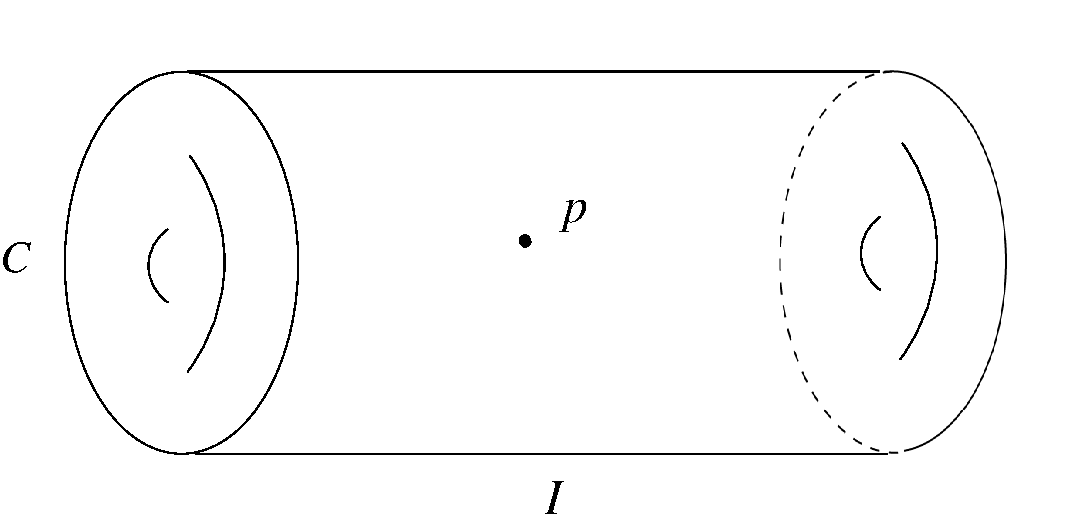
\includegraphics[width=0.75\linewidth]{figures/gla7-1.png}
\caption{A static 't Hooft line inserted at a point $p=y\times p_0$ in $I\times C$. Near this point, the solution of the Bogomolny equation has a prescribed singularity.（原文 Fig.~12）}
\label{fig:botampo}
\end{figure}

With 't Hooft lines included, things are more complicated
(\botampo). As we recall from section 第~\ref{sec:tophooft}~节, 't Hooft
operators create specified singularities in classical field
configurations. For an 't Hooft operator supported on the line
$\Bbb{R}\times p$, with some $p\in I\times C$, the singularity
will prevent us from  proving that the solution is a pullback from
$C$.  But for certain boundary conditions, a weaker vanishing
result still applies: the relevant solutions of \eqref{eq:oops}\ are
time-independent, that is, invariant under translations of
$\Bbb{R}$.

To explain this, recall that from the point of view of geometric
Langlands duality, the most important $A$-branes  are the branes
of type ${\CMF}$, supported on a fiber of the Hitchin fibration
with a flat Chan-Paton bundle of rank 1. They are $S$-duals of
zerobranes and hence are expected to be magnetic eigenbranes. As
explained in section 第~\ref{sec:mhbranes}~节, they are branes of type $(B,A,A)$,
i.e. the corresponding boundary conditions are compatible with two
linearly independent topological supercharges, suitable linear
combinations of which generate the topological supersymmetry of
the $B$-model in complex structure $I$ and the $A$-models in
complex structures $J$ and $K$.

When we consider BRST-invariant field configurations with
$(B,A,A)$ boundary conditions and an insertion of the 't Hooft
operator, we can distinguish between configurations which preserve
both fermionic symmetries and those which preserve only the
$A$-type  supersymmetry in complex structure $K$. In the latter
case, the broken supersymmetry generates an extra fermionic zero
mode that is not lifted by quantum corrections, since it is
generated by a symmetry, and will prevent such instantons from
contributing to any topological observables. (There may also be
other fermionic zero modes whose existence does not follow from
the fermionic symmetry.)  Hence, contributions of interest come
only from instantons that preserve both supersymmetries.

In fact, instantons with the requisite properties are
time-independent. One would guess this from the sigma-model, since
the $B$-model in complex structure $I$ has no non-trivial
instantons.  The result is also true in the context of the full
twisted supersymmetric gauge theory on $\Bbb{R}\times I\times C$,
even in the presence of static 't Hooft operators.  The most
general proof of this involves a moment map argument and will
appear elsewhere \cite{ref26}. Here we sketch another argument that is
adequate for the most important $(B,A,A)$-branes, such as branes
of type ${\CMF}$.

First we need a vanishing theorem for $\phi_1$, the component of
$\phi$ in the $I$ direction of $M=\Bbb{R}\times I\times C$. In any
classical instanton solution, $\phi_1$ will obey its second order
Euler-Lagrange equations, which can be deduced from the classical
action \eqref{eq:nuseful}\ and read % [WARN] 公式 \eqn\eqref{eq:zungo} 无编号或重复
\begin{equation*}
\tag*{(9.3)}
-D_\mu
D^\mu\phi_1+[\phi_\mu,[\phi_1,\phi^\mu]]=0.
\end{equation*}
 We suppose that
$\phi_1$ obeys Dirichlet or Neumann boundary conditions on each
brane; this is true for the most important branes.
 Multiplying  the equation by
$\phi_1$, taking the trace and integrating over space-time, we get
% 式 (9.4)
\setcounter{equation}{3}
\begin{equation}\label{eq:wungo}
\int d^4x\ \Tr\left( D_\mu\phi_1
D^\mu\phi_1+[\phi_1,\phi_\mu][\phi_1,\phi^\mu]\right)=0.
\end{equation}

Integration by parts produces no boundary terms because of the
assumed boundary conditions, and there is no problem with the
singularities associated with the 't Hooft operators because
$\phi_1$ is nonsingular near a static 't Hooft operator. Since the
integrand is negative-definite, the above identity implies that
$D_\mu\phi_1=[\phi_\mu,\phi_1]=0$, so that $\phi_1=0$ in the case
of an irreducible solution.

In this argument, we tacitly assumed that the integration by parts gives no
boundary term in the far past or future.  We do not know {\it a priori} that a supersymmetric
solution of the equations is time-independent.  However,
we at least assume that the desired solutions approach time-independent ``vacuum'' solutions in the
far past or the far future.  By first running the argument of the last paragraph for the
time-independent case, we learn that $\phi_1=0$ in each vacuum.  It then follows, since $W$ is
compact, that $\phi\to 0$ exponentially fast in the far past or the far future.  Hence, there is
no boundary term in the integration by parts used in the last paragraph to show that $\phi_1=0$
everywhere.

Now we want to show that a field that possesses the topological
supersymmetry of the $A$-model in both complex structures $J$ and
$K$ and also has $\phi_1=0$ is actually time-independent. The
supersymmetric equations of the $A$-model in complex structure $K$
are the equations \eqref{eq:oops}\ at $t=1$; those in the $A$-model in
complex structure $J$ are obtained from these by making a ${\cal
U}_1$ transformation $\varphi\to i\varphi$.  It is a short
exercise to write out the combined system of equations on
$M=\Bbb{R}\times I\times C$ and show that, if in addition
$\phi_1=0$, they imply that the fields are time-independent up to
a gauge transformation.

The time-independent supersymmetric fields can usefully be
analyzed in the more general context of $M=\Bbb{R}\times W$ with
static Wilson lines (without specializing to $W=I\times C$), even
though our argument that all relevant supersymmetric fields are
time-independent does not hold in this generality. When we
specialize to $M=\Bbb{R}\times W$, there is a further symmetry
${\EUT}$ of time-reversal invariance, acting as $s\to -s$ where
$s$ is a ``time'' coordinate on $\Bbb{R}$; ${\EUT}$ acts trivially
on $W$ and maps $(A,\phi)\to ({\EUT}^*A,-{\EUT}^*\phi)$. (This is
an example of the orientation-reversing symmetries discussed at
the end of section 第~\ref{sec:canonpar}~节.) The sign change of $\phi$ is needed
because ${\EUT}$ reverses the sign of the Hodge $\star$ operator
in \eqref{eq:nops}.

Therefore, we can consistently restrict ourselves to solutions
that are both time-independent and $\EUT$-invariant. In such a
solution, the $G$-bundle $E$ and connection $A$ are pullbacks from
$W$. Also, $\phi$ takes the form $\phi_0\,ds$, where $\phi_0$ is
an ${\rm ad}(E)$-valued zero-form on $W$.  The equations reduce to
% 式 (9.5)
\setcounter{equation}{4}
\begin{equation}\label{eq:bogeq}
F=\star D\phi_0.
\end{equation}
 Our orientation conventions are such
that in four dimensions, $\star(dx^0\wedge dx^1)=dx^2\wedge dx^3$,
and in three dimensions, $\star(dx^1)=dx^2\wedge dx^3$. The
equations \eqref{eq:bogeq}\ are the standard Bogomolny equations
\cite{ref105} for
supersymmetric or BPS monopoles\footnote{The name reflects the fact
that the basic supersymmetric monopole solution was also found in
\cite{ref106} as a solution of the second
order Yang-Mills-Higgs equations.} and have been widely studied,
for instance in 

\cite{ref107,ref108,ref109}.  A more familiar way to obtain the
Bogomolny equations is to look for solutions of the Yang-Mills
instanton equation on $\Bbb{R}^4$ that are invariant under
translations in one direction.

In this section, we will first analyze static 't Hooft operators
in the context of the standard Bogomolny equations \eqref{eq:bogeq}.  We
will show that they implement Hecke transformations of
$G$-bundles, as usually defined in the geometric Langlands
program.   This will involve studying BPS monopole solutions with
point singularities due to the 't Hooft operators.  Such singular
solutions of the Bogomolny equations have been studied first in
unpublished work by Kronheimer \cite{ref110}.  They can
arise as limits of smooth monopole solutions for larger gauge
groups 

 
\cite{ref111,ref112,ref113,ref114}, and from certain string theory brane
configurations \cite{ref115}, which have motivated more recent study in

\cite{ref116,ref117,ref118}. Then we will provide an
elementary introduction to Hecke modifications of $G$-bundles --
claiming neither novelty nor completeness from a mathematical
point of view!

In section 第~\ref{sec:extbog}~节, we will generalize the analysis to relax the
assumption of time-reversal symmetry. As we will see, in this case
the supersymmetric equations give a sort of complexified or
extended analog of the Bogomolny equations, which does not appear
to have been studied before. In the context of these extended
equations, static 't Hooft operators act by Hecke transformations
of Higgs bundles or in other words  of Hitchin pairs
$(E,\varphi)$. Hecke operators in this extended sense are natural
mathematically and have been considered before

\cite{ref119,ref120}.

Applications to the geometric Langlands program really depend upon
the extended Bogomolny equations and Hecke operators. We can
reduce to ordinary Bogomolny equations and Hecke operators only
when the boundary conditions (the choices of branes) ensure that
the Higgs field $\varphi$ vanishes. This is not the case for
typical applications.  However, we begin with ordinary Bogomolny
equations and Hecke operators and devote most of our attention to
them because this case is simpler and exhibits the main ideas.
